% #############################################################################
% This is Chapter 2
% !TEX root = ../main.tex
% #############################################################################
% Change the Name of the Chapter i the following line
\fancychapter{Background}
\cleardoublepage
% The following line allows to ref this chapter
\label{chap:back}

	The development of an algorithmic-based framework for optimization, applicable to architectural domains, requires a careful review over the current literature on \ac{BPO} practices and limitations. 
	
	Firstly, the \textit{ad-hoc} nature of the functions used for performance assessment in \ac{BPO} motivates the application of a special class of optimization algorithms, the derivative-free algorithms. Within this class, different categories emerge, emphasizing algorithms' different properties and search strategies. Each algorithm is able to potentially increase the effectiveness of an optimization process, depending on the characteristics of the considered problem. 
	
	Secondly, there are multiple approaches to optimization that might be considered. Generally, \ac{BPO} practices include the simultaneous optimization of multiple aspects. However, they often opt for simpler  specifications, often disregarding all but one of the initial considered aspects. 

	Finally, currently available architectural design optimization tools explore the parametric models produced in visual programming environments, such as Grasshopper and Dynamo. These graphical environments are implemented as plug-ins, which are tightly integrated with a \ac{CAD} and a \ac{BIM} tools, respectively. As a result, the connection between optimization tools and visual design workflows becomes seamless and friendlier. These optimization tools usually expose a \textit{ready-to-run} interface, which is very appealling to most \ac{BPO} practitioners~\cite{Cichocka2017SURVEY}.
	
% #############################################################################
\section{Derivative-Free Optimization}

	Different optimization algorithms can solve more or less efficiently specific optimization problems, depending on their characteristics. Particularly, classical gradient-based algorithms are very efficient solvers for optimization problems explicitly defined by mathematical formulations. This results from the fact that gradient-based algorithms explore information about the derivatives extracted from the mathematical formulation to guide the search for optimal solutions. However, when neither the mathematical form is easily available, nor is the information about the derivatives, it becomes necessary to explore other classes of algorithms. In these cases, the class of derivative-free algorithms is remarkably suitable for addressing these problems, as they do not use information about the objective functions' derivatives to find optimal solutions, instead, treating the objective functions as \textit{black-boxes} and guiding the search based on the result of previously evaluated solutions~\cite{Rios2013}.
	
	In architecture, it is often impossible to mathematically model the underlying objective functions for complex designs. Alternatively, architects use simulation tools as means to replace closed-form mathematical expressions that relate the design's parameters to the objective functions: simulation tools' results and other quantitative measures for different configurations of a design define the objective functions to optimize~\cite{Wortmann2016BBO}. Additionally, information about underlying objective functions is not easily attainable, often requiring excessive amounts of resources. The absence of information about objective functions prompts the need for algorithms that treat these functions as \textit{black-boxes}. One simple approach is to systematicly experiment with different parameter values until the best solutions are found, whereas a second, and more complex, approach is to use derivative-free optimization algorithms, also commonly referred to as black-box optimization algorithms within the architectural community~\cite{Wortmann2016BBO}. Despite its simplicity, experimentation-based approaches, such as Monte Carlo Sampling and Latin Hypercube Sampling~\cite{Giunta2003DOE}, might not always be advisable, particularly when dealing with time-consuming functions as is the case of architecture. In such cases, derivative-free algorithms might be more appropriate, yielding better solutions in less time.

	Building design's complexity has been raising for the past few years, leading to more complex objective functions, for which analytical forms are difficult to derive~\cite{Machairas2014}. For this reason, derivative-free algorithms are sought as useful tools to optimize designs, having been applied extensively to optimize building designs' manifold aspects. Among the numerous studies that apply derivative-free optimization algorithms to optimize building designs, we refer to the distinct works of Wortmann~\cite{Wortmann2016BBO,Wortmann2015AdvSBO,Wortmann2017GABESTCHOICE,Wortmann2017Opossum}, Evins~\cite{Evins2011,Evins2012MOO,Evins2013}, and Waibel~\cite{Waibel2018} which cover the optimization of various aspects, including, among others, the structural, the lighting, the thermal, the energy consumption, and the carbon-emissions. 
	
	For the past decades, the constant development and improvement of derivative-free optimization algorithms led to a diversified tools' gamut, each with its own characteristics and limitations. While the main ideas behind each algorithm's category seem to be more or less recognized throughout the architectural community, the lack of standards make it difficult to decide which definitions to convey~\cite{Rios2013, Wortmann2017ADO}. The currently most relevant classifications are: (1) the one presented by Rios et al.~\cite{Rios2013} that, based on the functions being used to guide the search process, classifies the algorithms into direct search or model-based algorithms; and (2) the classification provided by Wortmann et al.~\cite{Wortmann2017ADO}, which first subdivides the algorithms in two groups according to the number of solutions generated in each iteration, namely metaheuristics and iterative algorithms, and only then proceeds to classify iterative algorithms as direct search or model-based algorithms depending on the function that is used during the search. 

	This thesis will consider an approach similar to the one proposed by Wortmann~\cite{Wortmann2017ADO} by exploring the concepts of metaheuristics, direct-search, and model-based algorithms. Albeit the apparent chasm between these classifications, some algorithms draw ideas from distinct classes, thus emphasizing not only the blurred lines of such categorizations, but also the difficulties that lie with the definition of more standardized classifications. 
	
	The following sections describe each class and its intrinsic characteristics, proceeded by a brief comparison among them in light of the architectural design practice. 	

% ----------- Subsection
\subsection{Direct Search Algorithms}
\label{ssec:direct-search}

	Although there seems to be no precise definition for direct search algorithms~\cite{Kolda2003}, these are often identified as algorithms that iteratively~\cite{Kolda2003,Wortmann2016BBO}: (1) evaluate a finite sequence of candidate solutions, proposed by a simple deterministic strategy; and (2) select the best solution obtained up to that time. They are sought as valuable tools to address complex optimization problems, not only because most of them were proved to rely on solid mathematical principles, but also because of their good performance at initial stages of the search process~\cite{Rios2013, Wortmann2016BBO}. 
	
	The main limitations of the algorithms in this class is their performance deterioration with the increase on the number of input variables and their slow asymptotic convergence rates as they become closer to the optimal solution~\cite{Kolda2003}.

	Some examples of relevant direct-search algorithms include \ac{HJ}~\cite{Hooke1961}, \ac{NMS} method~\cite{Nelder1964}, SUBPLEX~\cite{Rowan1990}, \ac{DIRECT}~\cite{Jones1993DIRECT}, among others.
	
% ----------- Subsection
\subsection{Metaheuristics Algorithms}
\label{ssec:metaheuristics}

	In the original definition~\cite{Glover2003Metaheuristics}, these algorithms were solely based in the interaction between local improvement procedures, called heuristics, and higher-level strategies, called metaheuristics. On the one hand, heuristics are techniques that locate good solutions, but not necessarily the optimal, nor the correct solution, and that often consider the trade-off between precision and quality, and computational effort. On the other hand, a metaheuristic is an algorithmic framework that can be applied to different problems with a few modifications to add problem-specific knowledge~\cite{Glover2003Metaheuristics}, if so is desired. Moreover, a metaheuristic is a higher-level strategy that extends the capabilities of heuristics by combining one or more heuristic methods (referred to as procedures), while being agnostic to each heuristic. Metaheuristics are ``meta'' because they control heuristics.

	Throughout time, this class has grown to include any algorithm that includes simple heuristics to locate good solutions in complex design spaces, while considering the trade-off between precision, quality, and computational effort of the solutions. These algorithms often rely on randomization, and biological or physical analogies, to perform robust searches and to escape local optima~\cite{Glover2003Metaheuristics, Wortmann2016BBO}. Additionally, their non-deterministic and inexact nature confers them the ability to effortlessly handle complex and irregular objective functions~\cite{Wortmann2017GABESTCHOICE}, as well as, to easily adapt to \ac{MOO} contexts, or even to provide with domain-specific knowledge through the heuristics~\cite{Wortmann2017GABESTCHOICE}.
	
	Metaheuristics are efficient optimization algorithms when provided with sufficient amount of time to do the necessary objective function evaluations~\cite{Conn2009}. However, advantages can quickly become disadvantageous by simply changing the application context. This is the case of \ac{BPO} in the architectural practice, where each evaluation is a time-consuming task and the execution of thousands of evaluations rapidly becomes an infeasible scenario. Due to their stochastic nature, limiting the number of evaluations has severe repercussions both on the convergence and performance guarantees~\cite{Hasancebi2009}. 
	
	In the architectural design context, some of the most relevant metaheuristics algorithms include the \ac{PSO} algorithms, some evolutionary algorithms, such as \ac{GA} and \acp{ES}, and even local search algorithms like tabu search and simulated annealing. We refer the interested reader to~\cite{BlumRoli2003Metaheuristics,Glover2003Metaheuristics} for more details about these metaheuristics algorithms.

% ----------- Subsection
\subsection{Model-based Algorithms}
\label{ssec:model-based}

	Problems with time-consuming computer models and where sensitive information is expensive to collect can be approached effectively by model-based algorithms~\cite{Forrester2009SBO, Wortmann2016BBO}. These problems are characterized by the large time complexity associated with the computation of the values of the objective function and by the absence of previous knowledge about the objective function. Model-based algorithms are able to provide instant estimates of a design’s performance, by supplementing or replacing the original objective function by its approximation~\cite{Wortmann2016BBO}. This approximation, called the surrogate, is generated from a set of known objective function values, and is then used to determine the promising candidate solutions to evaluate next. These candidate solutions are then used to improve the surrogate and this process is repeated until a stopping condition is satisfied~\cite{Koziel2011}.

	Despite having a well-defined analytical form, which makes computations on the surrogate model more efficient than on the original objective function, the surrogate is only an approximate representation of the original function, and, therefore, must be constantly updated to guarantee a reasonable locally accurate representation~\cite{Koziel2011}. ~\Cref{fig:sbosexample} illustrates a surrogate that is accurate near the initial solutions. However, as we analyse solutions far from the initial ones, the accuracy of the surrogate model worsens.
	
	% Begin Figure: SBO Simple Example ----------------------------
	\begin{figure}
	\centering
	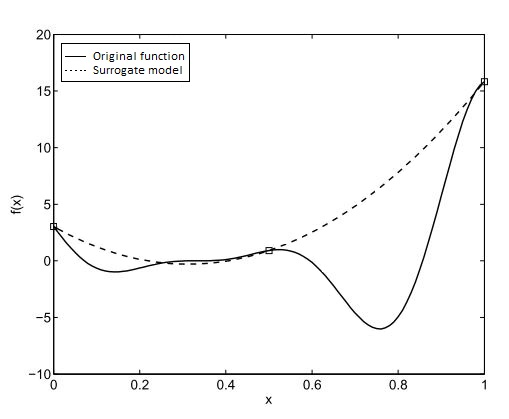
\includegraphics[width=8cm]{Images/Background/sbosexample.JPG}
	\caption{Original function and corresponding surrogate model, created based on three initial solutions (squares). This image was retrieved from~\cite{Koziel2011}.}
	\label{fig:sbosexample}
	\end{figure}
	% End Figure -------------------------------------------------------
	
	Nowadays, the existing plethora of techniques applicale to the generation of surrogate models, range from trust region methods to \ac{ML} techniques. These techniques can be used to create (1) local surrogates, i.e., models where the approximation to the objective function is built around a certain point, and (2) global surrogates, i.e, models where the approximation is generated from all the obtained points. Whilst the former relies on the construction of simple, partial models of the objective function, the latter relies on the creation of a full model. The creation of the full model, requires balancing the need for improving the accuracy of the model by exploring broader regions in the solution space, with the need for improving the value of the objective function by exploiting promising regions~\cite{Koziel2011}. This balance is determined by a strategy that selects the next promising solution to evaluate.
	
	Undoubtedly, the best feature of model-based algorithms is the reduction in the total optimization time. This is particularly relevant in the context of \ac{BPO}, where each simulation may take seconds, minutes, hours, days, or even weeks to complete. However, despite their benefits, the low availability and the technical knowledge frequently required to implement or incorporate these algorithms into optimization processes is not easily accessible to architects. Thus, despite the existence of different reports involving \ac{ML} techniques for the creation of full surrogate models~\cite{Koziel2011, Forrester2009SBO}, such as \acp{NN}, \acp{SVM}, \ac{RBF}, and \acp{RF}, among others, only a few have actually been applied in the context of architecture. This scenario is even more self-evident when we shift from the single- to multi-objective optimization context.

% ----------- 
\subsection{Comparison}
\label{ssec:comparison}

This section considers the applicability of different classes of derivative-free optimization algorithms for architectural design. The multidisciplinary character of building design raises distinct problems, ranging from well-behaved problems with simple, unimodal, convex functions to more ill-behaved problems with irregular, multimodal objetive functions~\cite{Wortmann2017ADO}. In addition to problem's diversity, the time complexity associated to function evaluations also becomes an important factor to consider when pondering each category's impact on \ac{BPO} problems.

	The problems' plethora within performance-based design is vast: a specific optimization algorithm may perform well for some problems and have a terrible performance in other problems~\cite{Wortmann2017GABESTCHOICE, Fang2017}. This idea resembles the ones captured in Wolpert's \acp{NFLT} for optimization, which state that any algorithm's worse performance over some classes of problems offsets its better performance in other classes. Because of the distinct nature of architectural design problems, the arguments herein provided are not necessarily applicable to other fields like science and engineering. 
	
	Inevitably, the same building design description might yield different problem descriptions according to the performance aspects being considered. Some algorithms might explore certain descriptions more effectively than others, for example, because the objective functions describing the lighting and structural behavior of a certain design may have completely different properties. In an attempt to exploit this property, \ac{BPO} practitioners often dedicate a small amount of their total time budget to test various algorithms and different setup parameters, before finally settling for an optimization algorithm~\cite{Hamdy2016}.	
	
	Regarding the different algorithms' categories, it is interesting to see the metaheuristics' popularity among researchers and practitioners. The main reasons behind the idolization of the metaheuristics are their: (1) inherent simplicity, (2) ease of implementation, and (3) wide applicability to different domains\todo{check if any other properties are relevant, for example in wortmann's works}~\cite{Wortmann2017ADO}. Unfortunately, other categories do not benefit from such properties, which is a limitation towards their application in architectural domains. For architecture, the major limitations to other categories lie in the absence of easy-to-use tools. Firstly, these tools are usually available as programming frameworks instead of integrated in architectural design workflows. As a result, to use the framework's optimization algorithms, architects often need some programming knowledge to create the scripts to integrate the algorithms into the design workflow. Unfortunately, since architects typically lack the required knowledge, they tend to struggle with the scripts production and, eventually, opt for using friendlier metaheuristics ready-to-use tools. Given this facts, it is not surprising that most of the existing building design optimization literature ends up focusing on the application of algorithms from the metaheuristics category~\cite{Hamdy2016, Nguyen2014, Evins2013}. 
		
	However, in the light of the \acp{NFLT}, the need for more short-term efficient optimization approaches fostered the development of tools exposing algorithms with different properties. Particularly, the plug-ins Goat\todo{CITE} and Opossum~\cite{Wortmann2017Opossum} enable the usage of algorithms from both direct search and model based classes. These tools expose optimization algorithms from the NLopt ~\cite{NLOPT} and RBFOpt\todo{CITE} frameworks, respectively, providing friendly, ready-to-use interfaces within Grasshopper\todo{Cite}, a visual programming environment that enables the parametric design and performance evaluation of building designs for different values of the parameters. For the past few years, few works have compared different algorithms using these tools with the ones available in metaheuristics tools, such as Galapagos \todo{CITE}, Octopus \todo{CITE}, Optimo\todo{CITE}, Silvereye\todo{CITE}, among others.
	
	Although the results may vary, in general, direct search and surrogate-based algorithms seem to be more effective than the metaheuristics ones in initial stages of the optimization process~\cite{Wortmann2017,Wortmann2016BBO,Wortmann2017GABESTCHOICE}. Even some metaheuristics algorithms can be very effective approaches for some optimization problems~\cite{Waibel2018}. 
One can explore these performance fluctuations to find the most effective optimization algorithm for a specific problem. This performance gain can be determining in the overall optimization time, especially, when complex and time-consuming simulations are involved. Indeed, several authors ~\cite{Wortmann2016BBO,Hamdy2016} suggest that the selection of the optimization algorithm should be based on the results of several tests with different methods for a fixed number of evaluations or a fixed amount of time. 

	Optimization is a useful tool to address both single and multi-objective problems. In architecture, most optimization applications focus on single-objective problems and cover the three different derivative-free algorithms classes. However, the same does not happen with multi-objective problems, with only one of the classes being extensively applied to \ac{MOO} building design: the metaheuristics~\cite{Hamdy2016}. The main reason behind metaheuristics popularity is their broader adaptability to both varying degrees of complexity and to different problem domains~\cite{BlumRoli2003Metaheuristics}.
	
	Recent developments in multiple surrogate-assisted \acp{MOEA} in the fields of science and engineering~\cite{Zapotecas-Martinez2016,Hussein2016} made it possible to decrease the number of expensive evaluations in \ac{MOO} problems. Generally, these techniques combine metaheuristics methods, which find more than one solution within a single execution, with surrogate models, which are approximations of the original objective functions. Diaz-Manriquez et al.~\cite{Diaz-Manriquez2016} provide a comprehensive overview of surrogate-assisted techniques for \ac{MOO} from the engineering perspective. 

	The following sections focus on the current \ac{BPO} practices both for \ac{SOO} and \ac{MOO}, the currently available tools, the advantages and disadvantages of each approach.
	
% #############################################################################
\section{Single-Objective Optimization}

\todo{O QUE FALAR AQUI ?? } 
?????

% #############################################################################
\subsection{Optimization Tools in Architecture}

	Most \ac{SOO} problems 

% ****** 
\subsubsection{Galapagos}

% ****** 
\subsubsection{Goat}

% #############################################################################
\section{Multi-Objective Optimization}

Due to the multiplicity of potentially conflicting goals involved in \ac{MOO} problems, the concept of optimality significantly differs from the one commonly used in \ac{SOO} problems. In \ac{MOO}, the best possible configuration for one objective is rarely the best configuration for all the other objectives as well, since these objectives are often contradictory. A possible way to define a solution’s optimality is through the Pareto optimality concept: a solution is considered to be Pareto-optimal if, given its objectives, it is impossible to improve an objective value without deteriorating the others. The solutions for which the previous property verify are said to dominate the other solutions from which it is possible to improve. For that reason, we say that the former ones are non-dominated, whilst the latter are dominated. In the context of \ac{MOO}, one is commonly interested in retrieving the set of non-dominated solutions, which is known as the Pareto Front (or Pareto Frontier). An example of a two-objective minimization problem is illustrated in ~\cref{fig:paretofrontier}. The two objectives are $f_1$ and $f_2$ and the solutions shown in orange are non-dominated. The optimization algorithm will try to find design solutions in the search space that lie on the Pareto Front.


% Begin Pareto-Optimization Figure -------------------------------------------------------
\begin{figure}
\centering
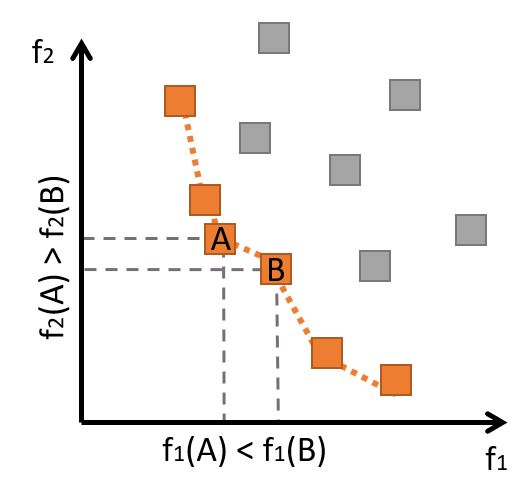
\includegraphics[width=5cm]{Images/Background/pareto-front.JPG}
\caption{Representation of the set of non-dominated (orange squares) and dominated (gray squares) solutions for a two-objective minimization problem. The Pareto front is composed of all the non-dominated solutions.}
\label{fig:paretofrontier}
\end{figure}
% End Figure -------------------------------------------------------



	According to the knowledge and level of expertise of the designers, \ac{MOO} problems might be approached differently. The following sections provide a more detailed description of the three main \ac{MOO} approaches.


% ----------- 
\subsection{Experimental Approach}

	The experimental or design of experiments approach is widely used in research and in practice to address both single and multi-objective problems~\cite{Fang2017}. Besides being intuitive and flexible, it can achieve a potentially better solution without having to deal with complex optimization algorithms. Sampling methods, such as Full-factorial, Monte Carlo Sampling, and Latin Hypercube Sampling ~\cite{Giunta2003DOE} are used to randomly generate different combinations of the design parameters, which are then evaluated. One advantage of having multiple solutions instead of just one is that the choice of the best solutions can be exclusively relegated to the architect, who analyses all the generated variations, and subsequently decides on the solutions he
thinks are the best (e.g., using preference articulation, pondering the conflicting criteria).

	Unfortunately this approach does not guarantee that good solutions will be found. In fact, in most cases input configurations are generated a priori and do not take advantage of any additional information. Consequently, the performance of previously evaluated design candidates is not used to guide the search towards the most efficient designs. Concretely, this means that because the information of previous design variations is not used in the process, useless candidate designs can be sometimes evaluated.
	
	On the other hand, given its simplicity and flexibility, this approach allows to easily assemble more complex processes which are capable of directing the search towards better design variations. For example, consider an optimization problem where an architect selects a sampling method to generate different design variations, which are then evaluated. After analysing the results, the architect may wish to explore design regions around the most promising solutions. In that case, he must limit the design variations to lie within the promising regions, by updating the problem’s definition. The redefined problem is then subsequently sampled and redefined until the architect is satisfied with the quality of the obtained solutions.
	
	Despite the constant need for manual intervention, the previous technique can be adapted to extract information about the design problem itself. Using an automated version of this technique, we are able to study the behavior of the different objective functions, when the input variables are changed. This process is known as \textit{sensitivity analysis}~\cite{Saltelli2007} and has been applied to multiple problems in the context of building design optimization~\cite{Tian2013}, either to enhance the performance of existing optimization algorithms, or to achieve better solutions.

	Overall, while it does not provide guarantees on the solutions’ optimality, this approach is simple, easy to use, and it is available in numerous tools. Moreover, although this process is not intelligent \textit{per si}, since the decisions are always made by the architect, it enables a more intelligent and informed design process, as it provides the full disclosure of the design variations generated, as well as their associated performance.

% #############################################################################
\subsection{A Priori Articulation Approach}

	This approach allows combining multiple objectives according to one’s preferences using an utility function \cite{Marler2004}. Among all the possible utility functions, the most commonly used is the weighted sum or linear scalarization \cite{Wortmann2017Opossum}. This function reduces multi-objective problems to single-objective by defining the objective functions to be the weighted sum of multiple objectives. The weights (or coefficients) represent the relative importance of each objective to the architect. These must be defined before
the optimization and, in general, they require expertise and experience, as this optimization approach is highly sensitive to the selected coefficients and that a different articulation of preferences might yield completely different results. The
final objective function is then provided to a \ac{SOO} algorithm, which tries to find an optimal (or near optimal) solution. In architecture, the ease of use, the availability,
the heterogeneity of ready-to-use \ac{SOO} tools (e.g. Opossum, Goat, Galapagos, Silvereye), and the time required by this optimization process are virtues of this approach.

	Overall, this approach enables a more intelligent design process because there is an algorithm that uses some knowledge about the previously evaluated solutions to guide the search towards optimal regions of the design space. However, because these algorithms are usually autonomous and independent of external
interventions, architects are often removed from the optimization loop, thus losing control over the design optimization process. Moreover, most of these algorithms
retrieve a single optimum and provide no other design options. This is a drawback~\cite{Cichocka2017SURVEY}, as the architect either complies to the retrieved solution or he must rerun the optimization with another articulation of preferences. Either
way, the optimization no longer provides enough information to make informed decisions.

% #############################################################################
\subsection{Pareto-based Approach}

	A more informative approach consists in the retrieval of a diverse and potentially heterogeneous set of Pareto-optimal solutions. When confronted with this set of optimal solutions, architects can compare different design options according to different performance aspects and make informed decisions about the compromises taken.

	When compared to previous approaches, one must consider (1) the number of function evaluations, which is larger due to the need to find a set of optimal solutions instead of focusing in a single one, (2) the visual representation of the solution space, which becomes problematic when the number of objectives is
greater than three, and (3) the modeling of the optimization problem itself, which directly impacts the quality of the solutions. 

	Notwithstanding the considerations above, a few studies concerning Pareto-based Optimization have emerged in the past years~\cite{Evins2013,Hamdy2016}. Indeed, the utility of Pareto optimization approaches has been recognized by architects as a useful decision support tool to building design \cite{Cichocka2017SURVEY}. Moreover, recent surveys show that even though scalarization approaches are are less time-consuming, they are not as desirable as Pareto optimization, since they do not aid in the decision-making process, nor
do they provide a clear trade-off between the different objectives involved \cite{Attia2013, Cichocka2017SURVEY}.
Despite the growing trend of Pareto optimization approaches~\cite{Evins2013}, the lack of relevant benchmarks comparing the performance of different \acp{MOOA} in architecture is evident, which justifies a comprehensive comparison among the performance of several algorithms applied to different problems in the
architectural context.

% #############################################################################
\subsection{Metrics for Multi-Objective Optimization}

% #############################################################################
\subsection{Optimization Tools in Architecture}

\subsubsection{Octopus}
\subsubsection{Opossum}
\subsubsection{Optimo}
